\documentclass[tcc, capa]{texucpel}

\usepackage[utf8]{inputenc}
\usepackage[T1]{fontenc}
\usepackage{verbatim}
\usepackage{amsmath}
\usepackage{graphicx} % para inserir figuras

\usepackage{microtype} % detalhes de justificação e espaçamento
\usepackage{nowidow} % evita que a última linha de um parágrafo mude de pag.
\usepackage{paralist} % lista sem o espaçamento de uma linha entre itens
\usepackage{booktabs} % 'rules' em tabelas
\usepackage{multirow} % Mágicas com tabelas
\usepackage{amssymb} % checkmark
\usepackage{icomma} % corrigir decimais (exceto unidades SI)
\usepackage{fourier} % muda a fonte de matemática pra colidir menos com arial
\usepackage{nameref}
\usepackage{verbatim}
 \usepackage{float}
\usepackage{siunitx}

\sisetup{
	detect-family = true,
	detect-shape = true,
	detect-weight = true,
	detect-mode = true,
	output-decimal-marker = {,},
	binary-units = true
}%



\newcommand{\esp}{ESP8266}
\newcommand{\esppci}{ESP-01}
\newcommand{\exehda}{EXEHDA}
\newcommand{\middleware}{\emph{middleware}}
\newcommand{\pic}{PIC}
\newcommand{\picm}{PIC18F4550}
\newcommand{\picf}{PIC18F}
\newcommand{\hc}{HC-05}
\newcommand{\meter}{\mbox{ubiMeter}}

\newcommand{\gambi}{\fontfamily{phv}\fontshape{n}\selectfont}
\newcommand{\media}{\(\textrm{\gambi{} Média (\si{\volt})}\)}
\newcommand{\desvio}{\(\textrm{\gambi{} Desvio Padrão}\)}
\newcommand{\maximo}{\(\textrm{\gambi{} Máximo (\si{\volt})}\)}
\newcommand{\minimo}{\(\textrm{\gambi{} Mínimo (\si{\volt})}\)}
\newcommand{\erromed}{\(\textrm{\gambi{} Erro médio}\)}
\newcommand{\erromax}{\(\textrm{\gambi{} Erro máximo}\)}

\unidade{Centro de Ciências Sociais e Tecnológicas}
\curso{Engenharia de Computação}
\nomecurso{Engenharia de Computação}
\titulocurso{Engenheiro de Computação.}

\title{Otimizando função de pontuação de docking molecular com uso de Support Vector Machine }

\author{de Campos}{Gianluca}
\vspace{1.2cm}

\advisor [Prof. Me.]{Mertins}{Luciano Edson}
%\coadvisor [Prof.]{Sobrenome}{Nome}

\keyword{Otimização}
\keyword{Estrutura}
\keyword{Avaliação}

\begin{document}
\maketitle 
\renewcommand{\advisorname}
{Orientador}          
%\renewcommand{\coadvisorname}{Coorientador}      %descomente caso tenhas coorientadora
\sloppy
\fichacatalografica
\folhadeaprovacao
%Opcional
%\begin{dedicatoria}
%\end{dedicatoria}

%Opcional
\begin{agradecimentos}
\textbf{Agradecimentos} \\
Em primeiro lugar gostaria de agradecer ao apoio de meus familiares por ser possível estar aqui estudando nesta instituição, dando o máximo de suporte possível para que eu pudesse estar aqui hoje.

Agradeço também aos colegas de turma, em especial ao Marcos, por me dar apoio na hora que mais precisei.

Também agradeço à colegas de trabalho, em especial Rodrigo Lima (vulgo Carioca) pela constante cobrança quanto aos prazos deste trabalho.

Em especial um agradecimento também ao meu Orientador por se disponibilizar para me ajudar ao longo deste curso, auxiliando nas difíceis tarefas, estudo e também pelo monitoramento delas, para que pudesse desta forma, concluir o trabalho.
\vspace{\baselineskip}
\end{agradecimentos}

%Opcional

\begin{epigrafe}{John Lennon}
"When I was 5 years old, my mother always told me that happiness was the key to life. When I went to school, they asked me what I wanted to be when I grew up. I wrote down ‘happy’. They told me I didn’t understand the assignment, and I told them they didn’t understand life."\\
\end{epigrafe}

%Resumo em Português (no máximo 500 palavras)
\begin{comment}
O processo de desenvolvimento de fármacos é normalmente algo custoso financeiramente, que demanda muito tempo e recursos para serem realizados, muitas vezes é feito por uma pessoa de forma manual. 

Esta questão pode ser melhorada, caso todo o processo fosse automatizado computacionalmente, mais especificamente tendo, um software que examine a estrutura de uma célula ligante e também faça a comparação entre suas similaridades com outra célula, esta sendo chamada de receptora, afim de ter um mapeamento de moléculas  que definem  ambas estruturas das  duas células e também a avaliação do quanto estão bem ligadas, para isto é aplicada uma técnica, chamada de Docking Molecular.

Os softwares existentes, utilizam o docking para este processo de avaliação, porém, possuem um precisão de acertos imprecisos ao lidar com grandes volumes de dados para serem avaliados. 
Para que possa ser melhorada a precisão desses softwares, deve ser feito uma otimização na função de avaliação usado nestes softwares e treina-la com deep learning, para que assim o processo de docking esteja trabalhando com melhores resultados. 
\end{comment}

\begin{abstract}
O processo de desenvolvimento de drogas medicinais é demorado, custoso e em grande parte manual.
Para melhorar e condicionar uma droga a um efeito desejado, use-se uma técnica chamada Docking Molecular, que consiste em realizar o atracamento entre uma estrutura denominada ligante e outra sendo uma receptora, onde o resultado do acoplamento, demonstrar o grau de afinidade da ligação entre as mesmas.
Esta técnica esta presente diversos softwares, que exibem design da estrutura das moléculas, onde é possível efetuar a manipulação e aplicar ajustes para então estimar resultados.
Para este trabalho, é proposto como solução aplicar, com auxílio de api's e bibliotecas da linguagem de programação Python, a técnica de aprendizado de máquina - Support Vector Machine(SVM). Fazendo uso de treinamento e teste, em bases de dados que contém informações de milhares de complexos do tipo ligante-proteína, com a finalidade de obter uma possível otimização no processo de predição de afinidade entre as estruturas.
Para avaliação de resultados, é realizada uma comparação com outro trabalho relacionado, utilizando a mesma métrica de avaliação (valor de erro médio quadrático - RMSE), bases de informações e quantidade de amostras.
Neste trabalho obteve um RMSE de 0.45 contra 0.74 ao aplicar a predição de afinidade no treino, e 1.97 contra 1.58 no teste.
Com isso uma melhora significativa pode ocorrer na classificação de estruturas desconhecidas, em trabalhos futuros, ajudando a diminuir o número de informações necessárias passadas para avaliação de possíveis fármacos alvo que podem ser compatíveis.
\end{abstract}

\begin{englishabstract}
  {Titulo do Trabalho em Inglês}
  {Algorithm, Optimization, Evaluation}  
  
The process of developing medicinal drugs is time-consuming, costly and largely manual.
To improve and condition a drug to a desired effect, use a technique called Docking Molecular, which consists of carrying out the mooring between a structure called a linker and another being a receiver, where the result of the coupling, demonstrate the degree of affinity of the bond between them.
This technique is present in several softwares, which show the structure design of the molecules, where it is possible to perform the manipulation and apply adjustments to estimate the results.
For this work, it is proposed as a solution to apply, with the help of api's and libraries of the programming language Python, the machine learning technique - Support Vector Machine (SVM). Using training and testing, in databases containing information from thousands of ligand-protein complexes, in order to obtain a possible optimization in the process of predicting affinity between structures.
For evaluation of results, a comparison is made with other related work,
Thus a significant improvement can occur in the classification of unknown structures in future work, helping to decrease the number of information needed to evaluate possible target drugs that may be compatible.

\end{englishabstract}

%Lista de Figuras
\listoffigures

%Lista de Tabelas
\listoftables

\begin{listofabbrv}{RFCOMM}
		\item[UCPel] \textit{Universidade Cat\'olica de Pelotas}
        \item[CAPRI] \textit{Critical Assessment of PRedicted Interactions}
        \item[RMSE] \textit{Root Mean Square Deviation}
        \item[API] \textit{Aplication Programming Interface}
        \item[SVM] \textit{Support Vector Machine}

        
        
\end{listofabbrv}

%Sumario
\tableofcontents

\chapter{Introdução}
Ao ser desenvolvida uma nova droga é necessário estudar as propriedades químicas e analisar a composição estrutural das moléculas, o processo de desenvolvimento é bem custoso e demorado, pois leva tempo para poder realizar testes e avaliar resultados,que são feitos em vitro e examinados em laboratório \cite{prnasciutti2012}, sendo em grande parte manual e dependente de um ser humano.

Por consequência disso é comum que seja utilizado softwares que analizam estruturas celulares e apliquem técnicas específicas da área de biomedicina para testes e avaliações simuladas computacionalmente, como por exemplo as ferramentas baseadas no princípio da técnica de docking molecular.
Um exemplo destes é o pacote de softwares open-source Autodock-Tools \cite{autodocktools}, que possuem programas que vão desde manipulação de e visualização da estrutura de possíveis fármacos a nível molecular (CADD), até ajuda a estimar o comportamento que duas estruturas realizam ao se juntarem \cite{trott2010autodock}.
Com isto o uso destes tipos de softwares, possível poupar tempo e diminuir o custo de recursos no desenvolvimento de fármacos.

Esses detalhes são importantes para aplicar o docking, pois trazem bastante informação ao realizar o estudo do comportamento entre duas estruturas celulares, que geralmente costumam ser um sequenciamento de DNA ou uma proteína.%\textbf{REF} % citar exemplo

Este comportamento é útil para o desenvolvimento de fármacos, podendo ajudar a estudar inibidores de um vírus por exemplo,  onde ao aplicar a técnica de docking foi possível descobrir substâncias que pudessem inibir o vírus Influenza\cite{ishikawa2011binding}.

O objetivo que se tem em aplicar a técnica de docking é analisar duas estruturas, uma considerada ligante e outra receptora, junta-las de forma que ocorra a melhor conformidade de encaixe possível, sendo a partir disto, possível de analisar as propriedades em comum e estuda-las.

Para poder aplicar o docking é necessário conhecer a molécula ligante, qual o receptor que seria qual estrutura ela irá se ligar (proteína ou DNA). Ao conhecer as estruturas, é avaliado qual o melhor ponto em que serão encaixadas, a quantidade de energia que será liberada ao ocorrer esta ligação e com isto qual o grau de afinidade entre a estrutura ligante receptora. Para isto é considerado o princípio da minimização energética, que prevê que quanto menor a energia, melhor conformidade \cite{kitchen2004docking}.

Com o passar dos anos, novas tecnologias foram surgindo, tanto a área da biomedicina quanto na computação,trazendo melhores hardwares e softwares, em razão disso os programas que realizam docking hoje em dia tem cada vez maior capacidade para processamento, permitindo que seja obtido melhores resultados, desempenho e maior riquezas de detalhes ao explorar uma estrutura celular.

Com essa evolução computacional, softwares começaram a aplicar utilizar técnicas de aprendizado de máquina para calcular e estimar resultados da função de pontuação.
Tendo diversos algoritmos empregados como; algoritmo genético \cite{holland1975adaptation},  Simullate Annealing \cite{kirkpatrick1984optimization} ,  algoritmo genético de Lamarca \cite{morris1998automated},  MonteCarlo \cite{caflisch1992monte} entre outros que foram tiveram evoluções ao longo dos anos. 

Dependendo do algoritmo utilizado, a precisão do resultado pode variar, assim como seu desempenho e rapidez para gera-lo.
Com a evolução da área computacional, novos estudos são feitos para obter dados com melhor desempenho, em particular a Deep Learning tem se mostrado útil para vários estudos na área de biomedicina conforme avaliado por \cite{korotcov2017comparison} e \cite{mamoshina2016applications}, esta técnica basicamente consiste em treinar a máquina, para que ela possa classificar algo em grande escala afim de se obter da melhor forma possível  os resultados.

Também  pode ser aplicado, como mostra \cite{ballester2010machine}, a técnica de florestas aleatórias para prever a afinidade de complexos de proteínas e ligantes ao utilizar bases de dados para treinamento e teste.

Existem diversas técnicas para serem empregadas a softwares de Docking, neste caso é interessante saber o que e como pode ser melhorado o mesmo, pois este será o trabalho da inteligência artificial, identificar padrões, aprende-los e predizer resultados.

\section{Objetivo do trabalho}

Este Trabalho aplica uma técnica de aprendizado máquina (SVM) com a finalidade de prever a afinidade de complexos ligante-proteína. Para isso foram utilizadas bases de informações (data-sets), \cite{wang2004pdbbind} sendo utilizadas para aplicar treinamento e teste. 
Como objetivo secundário foi feito uma comparação de resultados com o artigo de \cite{ballester2010machine}, onde o mesmo utilizou a técnica de florestas randômicas (random forests).
Com isso será possível demonstrar o índice de acertos previstos e a eficácia entre duas técnicas distintas  de aprendizado de máquina, utilizando as mesmas métricas para avaliação e bases de informações.
Com os resultados apresentados, o aprendizado de máquina ajuda a diminuir o número de levantamento de informações necessárias para poder ser feita a  avaliação de possíveis fármacos alvos a serem estudados

\section{Organização do texto}
Este trabalho tem capítulos divididos da seguinte forma.

O Capítulo 2 abrange o referencial teórico sobre o qual será desenvolvido o trabalho de conclusão de curso, em específico, explicando sobre a definição do que seria o docking, como é realizado o processo de docking, o contexto de onde está inserido, comentado brevemente sobre aprendizado de máquina, as técnicas existentes e bases de dados para treinamento e teste.

No Capítulo 3, é apresentado como será realizado o estudo e otimização da avaliação de resultados do docking molecular ao aplicar a técnica de SVM, contendo uma descrição dos componentes necessários para validar sua implementação.

No Capítulo 4, será descrito os resultados obtidos deste trabalho, sendo feito uma comparação com uma implementação utilizando Random Forests, descrevendo suas vantagens e desvantagens com o SVM.

Por fim, o Capítulo 5, falará sobre uma visão geral de todo o trabalho, traçando perspectivas para possíveis implementações futuras.

\chapter{Fundamentação Teórica}
Este capítulo faz uma breve revisão teórica sobre os assuntos necessários para a entender o processo de docking molecular  e aprendizado de máquina.

\section{Docking Molecular}
No final da década de 1980, surgiam os primeiros softwares que realizavam o processo de docking molecular, possibilitando desta forma trazer uma visão mais detalhada das estruturas. Com isso foi possível manipular as moléculas e otimizar as células com mais facilidade e simular com maior precisão, permitindo mais rapidez ao realizar testes virtuais.

Para realizar o docking, é necessário realizar o mapeamento das proteínas que irão se ligar, isso serve para prever os melhores pontos para que as moléculas se liguem, e conhecendo assim o ponto com melhor conformidade e energia que será gasta para a união. Isto pode ser visto na figura 1, onde mostra duas protéinas realizando  docking e consequentemente gerando inúmeros pontos de conformidade.

      \begin{figure}[!htb]
	\centering
 \cite{xue2015protein}
    \caption{Exemplo de dockagem entre duas proteínas}
    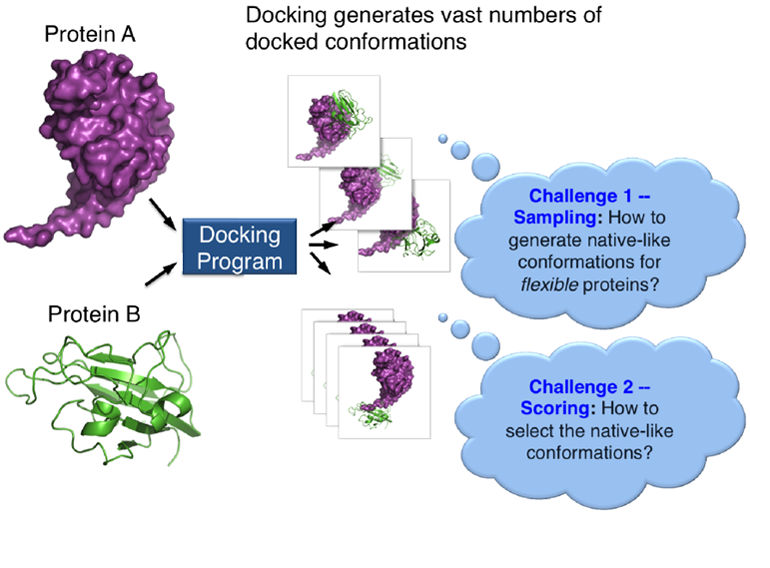
\includegraphics[width=10cm]{imagens/mostra_docking.png}
	\end{figure}
    
Tendo como objetivo analisar e prever a melhor conformidade entre duas estruturas celulares, conhecendo toda a região das moléculas das proteínas, ao aplicar o docking é possível descobrir a afinidade de ligação que estas duas moléculas possuem entre si, sendo assim estimando o melhor encaixe.
Ao ocorrer uma ligação, será liberado uma certa quantidade de energia, esta energia é importante para medir a conformidade da união entre duas moléculas (ligante e receptora).
Para realizar a medição, é utilizado funções de pontuação (score functions), focadas na minimização energética, que  segundo \cite{kitchen2004docking} e \cite{lybrand1995ligand}, chegaram a conclusão de que, quanto menor a energia gasta entre duas moléculas, melhor será sua a conformidade na união. 

Dependendo da estrutura que é analisada com o docking, torna-se possível criar uma substância capaz de inibir a molécula receptora, no caso de um inibidor de vírus por exemplo. \cite{ishikawa2011binding}

Com essa manipulação nas estruturas celulares, é possível destrinchar vários assuntos, pesquisas e artigos sobre os comportamentos de células e proteínas.
Esses exemplos são triviais para o estudo do comportamento das composições químicas das células para fazer medicamentos na área da biomedicina. 
Em geral é a técnica de docking molecular é utilizada para desenvolver estruturas de células diversas; vírus de doenças, medicamentos,DNA e tudo que envolva fármacos. 

Muitos softwares já obtiveram resultados positivos ao utilizar docking, conforme mostrado na tabela 1 abaixo, onde é listado exemplos destes softwares.
\begin{table}[h]
\centering
\caption{Softwares bem sucedidos ao utilizar docking molecular \cite{sliwoski2014computational} }

\begin{tabular}{@{}|c|c|c|@{}}
\toprule

Software & Alvo                   & Estudo                                                   \\ \midrule
Seed     & Plasmepsin             & Uma das causas da malária                                \\ \midrule
FlexX    & Fator de Edema Anthrax & Inibidor do edema                                        \\ \midrule
Glide    & Citocromo P450         & Deixa substâncias em formas hidrosolúveis         \\ \midrule
Surflex  & Topoisomerase I        & Otimização de anti-cancerígeno                           \\ \midrule
Dock     & Imunofilina F506       & Inibidor de calcineurina \\ \bottomrule
\end{tabular}
\end{table}

Para \cite{rodrigues2012estrategias}, o objetivo principal que se tem ao aplicar docking é; aprimorar o processo de busca de novos candidatos a fármacos e acelerar o processo contínuo do seu planejamento. 
Todos os fatores como as propriedades químicas das moléculas auxiliam a compreender de qual maneira se comportará as células, quais os tipos de ligação que podem ser utilizados como; proteína-ligando, proteína-DNA, proteína-proteína. Isso pode influenciar na abordagem de docking e afetar o desempenho nos softwares utilizados, ao serem aplicadas funções de pontuação.

Quanto a abordagem, existem duas formas diferentes de realizar o docking, que pode ser classificado como Docking Rígido e Docking Flexível.

No docking rígido os pontos de união de uma molécula ligante e receptora são mais limitados, isso se deve ao fato de existir uma menor liberdade em manipular as moléculas de uma célula, ou seja, a molécula ligante será rígida assim como o receptor. Consequentemente isso acaba resultando em maiores pontos a serem estimados para realizar a união de uma forma compatível. \\
Isso pode aumentar a precisão de acertos, já que existe vários pontos a serem avaliados e qual deles terá menor energia para realizar o acoplamento \cite{pagadala2017software}. 
Já no Docking Flexível, a molécula ligante pode ser manipulada com total liberdade ao tentar se acoplar no receptor,  este que continuará sendo rígido. O número de pontos a ser estimado será menor por ser ajustado a molécula ligante ao receptor rígido.
Geralmente é utilizado esta abordagem após ser feito o docking rígido, orientado o melhor resultado estimado anteriormente para que desta forma tenha-se uma boa conformidade, isto é ilustrado na figura 2.


      \begin{figure}[!htb]
	\centering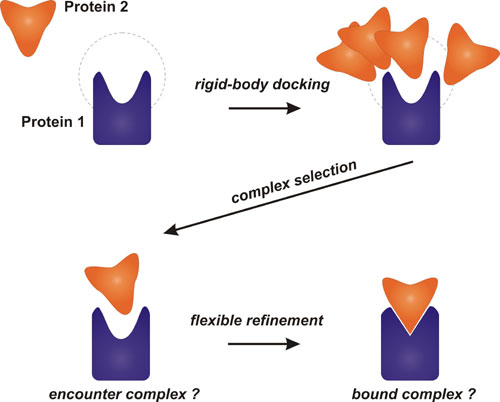
\includegraphics[width=10cm]{imagens/rigid_flexible.jpg}
	\caption{Docking Rígido com refinamento flexível}
	\end{figure}

\section{Função de Pontuação}
O aprendizado de máquina se tornou algo bem comum ao ser aplicado em diversas áreas da computação, ao ser aplicado em software deve ser levantado os pontos que são relevantes para o processo de docking.

Nos softwares de docking são utilizados algoritmos para gerar funções de avaliação para estimar o gasto energético durante a união entre moléculas, como por exemplo algoritmo genético \cite{holland1975adaptation}, Simulate Annealing \cite{kirkpatrick1984optimization} ,  algoritmo genético de Lamarca \cite{morris1998automated},  MonteCarlo \cite{caflisch1992monte}.

Estes algoritmos estão constantemente sendo evoluídos e até substituídos para obterem mais eficácia ao estimar grandes volumes de dados com um desempenho melhor.
Portanto, é possível dizer que ao melhorar a precisão desta função, é possível otimizar o processo de docking molecular consideravelmente.

\section{Software - Autodock Tools e Vina}

Um dos softwares mais populares utilizados por pesquisadores e cientistas da área é o Autodock Vina \cite{trott2010autodock}, que veio como parte do software dos mesmos criadores do Autodock Tools.

A maioria dos pesquisadores costumam realizar diversas modificações através deste software, utilizando o pdt (protein docking tools) para manipular a estrutura, adicionar ligantes e parâmetros extras, remoção de átomos de água, escolher pontos para simulação de interações, otimização e desenvolvimento de proteínas.

Nestes softwares, é possível visualizar os átomos do complexo em 3D, sendo exibidas informações das coordenadas graficamente, permitindo assim reconhecer a posição de cada ponto da estrutura, e então manipular as moléculas de um determinado complexo, com o objetivo de poder estimar a energia gasta para realizar o acoplamento. 

Após ser executado o processo desejado é salvo em um arquivo com formato .pdbqt, que será lido pelo software Vina. Este mesmo é encarregado de calcular e estimar os melhores pontos de interação para ser realizado o docking, que exibe em Kcal/s a afinidade dos melhores resultados.
Após adicionar ligantes a um determinada região de interesse (sítio de união), pode ser salvo em um arquivo .PDBQT, que irá conter informações referentes ao posicionamento dos átomos, que será lida pelo Vina, como mostra na figura abaixo.

      \begin{figure}[H]
	\centering
	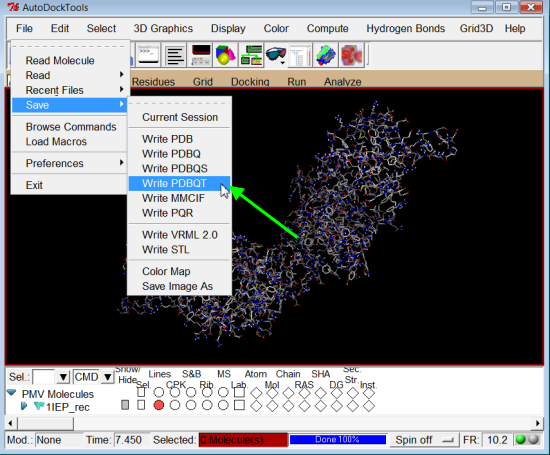
\includegraphics[width=0.90\linewidth]{imagens/Autodock.png}
	\caption{Exemplo de complexo}
	\end{figure}

Este é o procedimento utilizado pelos cientistas e bio tecnólogos ao utilizar estas ferramentas, logo após ser feita esta triagem simulada, é escolhido por especialistas os melhores resultados estimados pelo Vina, após diversos testes e assim feita a triagem em vitro, onde é tirada a prova real da qualidade das ligações.

Uma excelente métrica que diversos pesquisadores utilizam para testes e avaliações, é através do cálculo de desvio de raiz quadrada médio (RMSE), pois é possível comparar o overfiting no treinamento e teste.

\section{Técnicas de Aprendizado de Máquina }
%Falar sobre deep learning, svm, florestas aleatorias algoritmo genético e todas ténicas que foram utilizadas anteriormente em softwares
O foco será direcionado para o estudo de uma das técnicas de Inteligência Artificial na literatura, em específico uma delas; SVM, onde é possível utiliza-la para treinar os algoritmos para previsão e definição dos melhores resultados possíveis. 

Começando pelo pelo básico da IA, temos o aprendizado supervisionado e não supervisionado, dentre estes são utilizados funções de classificação e agregação que são muito limitadas para serem exploradas em um volumes de dados muito grande.% Citação
Para estudar o comportamento de uma célula é necessário fazer um mapeamento de sua estrutura para compreender suas peculiaridades e comportamentos. 

Tal processo é muito custoso, levando muito tempo gasto para exibir resultados, dependendo do poder de processamento e da técnica de machine learning utilizada (SVM, Algoritmo Genético,Random Forests).

Para fazer a máquina explorar e buscar informações referentes a composição das moléculas, será requerido bases de dados (data-sets), que irá conter os dados necessários para efetuar treinos e testes. 

Existem diversos softwares que utilizam técnicas de IA, cada um leva em consideração qual aspecto do docking deve ser melhorado. Abaixo é falado sobre alguns desses aspectos, segundo \textbf{\cite{khamis2015machine}}.

\textbf{(1)Poder de Pontuação:} Refere-se a habilidade de estimar diferentes poses de ligação para um determinado complexo de ligante-proteína. Com isso é possível fazer uma correlação para encontrar valores comuns e possivelmente prever diferentes resultados de afinidade.

\textbf{(2) Poder de Ranqueamento:}
É responsável por prever o valor mais próximo de energia gasta por cada complexo.

\textbf{(3)Poder de Docking:} Capacidade de identificar a melhor pose de conformidade para um dado ligante, através de um conjunto de poses geradas mostradas.

\textbf{(4)Poder de escaneamento:} Capacidade da função de pontuação descobrir e identificar os falsos positivos em uma determinada proteína alvo, junto a diversos conjuntos de moléculas distintas.

O foco deste trabalho foi estudar uma maneira para otimizar o poder de ranqueamento de docking, ou seja, ser capaz de avaliar e estimar qual o melhor resultado para uma estrutura de um determinada ligação ligante-proteína possa se encaixar, prevendo a afinidade ideal correspondente.

Para este caso em específico,\textbf{\cite{ballester2010machine}} utilizou florestas aleatórias e obteve um resultado satisfatório pois compreende um bom desempenho ao utilizar um grande volumes de parâmetros e informações predispostas em uma base de dados bem conceituada PDBBind \cite{wang2004pdbbind}

\subsection{Random Forests}
Conforme visto na literatura, o desempenho das demais técnicas dependem da performance de execução dos diversos recursos computacionais empregados, ou seja, partindo do pressuposto da utilização da técnica de florestas aleatórias, não será necessários exímios recursos e processamento para melhores resultados, é evidente que quanto mais vezes for treinado e melhor descritos os parâmetros, a eficácia será maior.

Dado o trabalho de \cite{ballester2010machine} como exemplo foi necessário fazer validações dos data-sets e criar estruturas específicas para comportamento de átomos,ligantes e proteínas para poder aplicar treinamentos nas data-sets.

As florestas aleatórias utilizam isso isso e aquilo, do qual é possível criar arquivos com n-features e recursos, para melhor compreendimento de como funcionará as florestas aleatórias, será explicado na seção de metodologia deste trabalho. 

Porém o uso desta técnica pode acarretar o overfiting devido a alguns fatores, que pode ser visto a seguir na seção de resultados.

\subsection{Support Vector Machine}

A técnica de máquina de vetores de suporte, denominada SVM, utiliza aprendizado supervisionado e é capaz de reconhecer padrões realizando classificação ou regressão. Esses padrões são reconhecidos através de exemplos que contenham parâmetros de entrada e um parâmetro de saída, este sendo chamado de Label.

O svm separa os padrões que considera similares, e os coloca em uma classe específica, com isso ele cria modelos que ao serem treinados são capazes de predizer a qual classe um novo exemplo pertence.\cite{boser1992training}

Um clássico exemplo para demonstrar em prática o SVM, é utilizando o data-set de Íris do \cite{fisher1936use}, onde é separado em diferentes classes cada uma das espécies de flores (Iris-Virginica,Iris-Versicolor,Iris-Setosa), acordo com o tamanho e comprimento. 

    \begin{figure}[!htb]
	\centering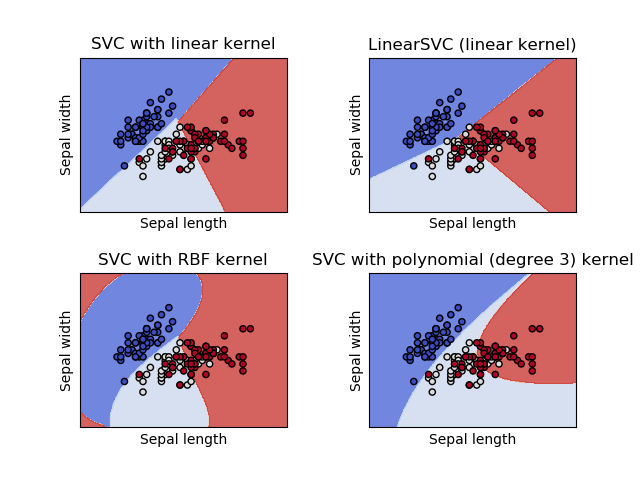
\includegraphics[width=15cm]{imagens/exemplo_svm.png}
	\caption{Classificando por comprimento e largura}
	\end{figure}

Ao analisar a figura é possível perceber que existe uma maior precisão de acertos de amostras ao utilizar diferentes tipos de Kernels.

Estes kernels possuem uma função específica, da qual são responsáveis por realizar a separação dos modelos do SVM, e existem diferentes tipos; linear,gaussiano,polinomial e sigmóide, sendo o mais comumente empregado o Gaussiano por ser capaz de analisar as bordas mais suavemente. %referência,

Por conta disto, este trabalho optou-se em utilizar o kernel Gausiano do SVM, descrito como RBF (radial basis function) 
por trazer o melhor resultado para prever a afinidade dos complexos.
As informações presentes nas bases de testes e de treino foram armazenadas em um data-frame, onde a afinidade do complexo constituem os labels e de resto os parâmetros de entrada. 

Para cada todos esses parâmetros de entrada deve propor uma saída (Label),  com isso o SVM irá realizar um treinamento utilizando uma análise de regressão utilizado o Kernel Gausiano como função principal.
Após ser realizado o treinamento é hora de predizer um valor para afinidade de acordo com os parâmetros informados.

\chapter{Metodologia}
Para este trabalho foi proposta uma alternativa ao RF-Score, algoritmo proposto por \cite{ballester2010machine}, sendo utilizando os mesmos dados das data-sets com a justa finalidade de comparação, buscando otimizar os resultados  de treino e teste, ao aplicar uma outra técnica de machine learning, Suporte Vector Machine (svm), com a finalidade de resolver os problemas presentes na implementação de floresta aleatória.

Em primeiro momento o foco será estudar os componentes necessários para realização de docking e  fazer uma revisão bibliográfica dos recursos necessários para realiza-lo, tais como informações relevantes que podem influenciar resultados e previsões para treinamentos e testes. 

Esta revisão tem como objetivo se aprofundar nos temas que envolvem todo o processo de docking como onde é aplicado, qual o processo para ser executado, as ferramentas, requisitos necessários  e saber quais os resultados esperados computacionalmente.

A parte de aplicações refere-se ao uso de docking e para o que é útil,  em especial o que seria necessário para desenvolver algum fármaco.

O processo de realizar docking através de softwares ajuda a entender como ocorre o funcionamento desta técnica, com isso é possível ter uma estimativa de quais são os requisitos e resultados esperados que serão avaliados computacionalmente.

Após ser estudado o docking foi realizado uma pesquisa a respeito da área de aprendizado de máquina, buscando especificamente o conhecimento da técnica de florestas aleatórias e SVM, que aborda temas como o a classificação das estruturas de proteínas bem como a predição dos melhores pontos estimados do docking.

Também foi feito um levantamento das ferramentas existentes; de quais ferramentas (softwares) são utilizados e quais foram as otimizações das funções de avaliação que tiveram ao longo dos anos segundo os benchmarks.

Assim como também testar e utilizar softwares,bases de dados, api's e frameworks de linguagens de programação, especificamente o módulo sklearn \cite{scikit-learn}, junto a linguagem de programação Python, que auxiliam no desenvolvimento e treino do aprendizado de máquina.

\section{Criação de Data-sets}
Conforme dito anteriormente, é necessário ter exemplos prontos, com parâmetros de entrada e saída para poder aplicar o treinamento e teste em um dado algoritmo de aprendizado de máquina.
Esses exemplos irão estar presentes em uma data-set, que contém diversas informações referentes a uma determinada amostra, quanto maior a quantidade de amostras melhor será o resultado.

É necessário baixar bases de dados em formatos de arquivo .pdb, que podem ser baixadas através do site (PDBBind). Essas bases contêm todas as informações necessárias para conhecer a estrutura das proteínas, ligantes e DNA. 
O uso dessas bases será de extrema importância,pois ao utiliza-la será possível aplicar treinamento e com isso estimar resultados no ao realizar um teste. 

Para este trabalho, os data-sets são organizados da mesma forma que \cite{ballester2010machine}, com o objetivo de realizar uma comparação entre estas duas técnicas de aprendizado de máquina, onde serão visto os resultados no Capítulo 4.

Essas bases contém complexos de proteínas-ligantes, e foram validadas com uma série de critérios descritos por \cite{cheng2009comparative}, pois as informações são muito heterogêneas, até mesmo para um processamento de técnicas de machine learning. 
Segue abaixo estes critérios adotados para criação desta base:

\begin{enumerate}
\item Apenas o complexos proteína-ligante cujas estruturas são determinadas através de difração de cristal foram considerados. Cada estrutura qualificada como complexa, deve ter uma resolução global melhor do que ou igual a 2,5 Å. Além disso, tanto a proteína como o ligando precisa estar completo na estrutura cristalina.
\item Preocupações sobre a qualidade dos dados de ligação. Apenas o complexos proteína-ligante com constantes de dissociação conhecidas (Kd) ou constantes de inibição (Ki) foram consideradas. Além do que, além do mais, tanto a proteína como o ligante utilizado no ensaio de ligação tem que corresponder exatamente aos usados na determinação da estrutura.
\item Preocupações sobre os componentes dos complexos. Somente os complexos de proteína-ligante ligados de forma não covalente foram considerados. Cada complexo qualificado deve ser formado por um molécula de proteína e uma molécula de ligando de uma maneira binária. Em outras palavras, não deve haver vários ligantes ligados nas proximidades de um local de ligação comum. O ligando molécula não deve conter elementos incomuns, como como Be, B, Si e átomos de metal.
\end{enumerate}

Para aplicação deste estudo foram utilizadas estas duas data-sets, uma chamada de refinada, que será utilizada para treinamento e outra chamada core que será utilizada para teste. 
A base refinada originalmente continha cerca de 1300 linhas de exemplos com os parâmetros descritos anteriormente, porém foram retirados e separados em 3 clusters com 65 complexos da mesma, que acabou sendo utilizada para o teste, que será chamada de core. Logo existem  2 datasets, um para treino com 1105 amostras (refinado) e outro para teste com 195 amostras para teste.


\section{Definição de Parâmetros}
%ainda não terminei
%Explicar sobre os labels e parâmetros utilizados para teste e treino do SVM.
%O que são as afinidades (pdbaff), distância euclidiana (6.6,6.7) e qual label (PDB) utilizado.

Seguindo o exemplo de \cite{ballester2010machine}, serão coletados a afinidade, de cada complexo dos arquivos presentes na base do PDBbind, será calculado a distância euclidiana entre as interações dos átomos de C,N,O,F,P,S,Cl,Br,I (somente daqueles) que compõem a estrutura do ligante e da proteína.

Um parâmetro na data-set será responsável por identificar a qual proteína é correspondente, ou seja, o Id do complexo (11gs por exemplo).

Para a afinidade é utilizado as constantes Kd(constante de dissociação), Ki (constante de inibição) e IC. Dependendo da estrutura só será informada alguma destas constantes, com é atribuído como valor de afinidade o resultado do -log10 K, sendo K a constante que estiver presente.

Para a distância eucliana de cada átomo será utilizado 36 campos de parâmetros que representam a distância entre um e outro, por exemplo a distância entre o átomo C e N representa um valor, C e O também e assim sucessivamente, resultando em 36 valores. 


\section{Bibliotecas e API's para SVM}

Falando um pouco sobre as ferramentas necessárias para construir o algoritmo de machine learning e avaliar resultados.

\subsection{Python}% Muito COPY PASTE MUDAR UM POUCO

A linguagem Python, versão 3, é de alto nível, com ênfase em manter o código legível e fácil de entender,  expressando programas em poucas linhas de código quando é comparada a programas feitos em outras linguagens.

Foi idealizada e inicialmente implementada por Guido van Rossum, na década de 80. Hoje, sua licença é administrada pela Python Software Foundation,\cite{pythonfundation} que permite seu uso inclusive para fins comerciais, e seu desenvolvimento é mantido por uma comunidade, uma vez que a linguagem é open-source.

Python é uma linguagem de tipagem dinâmica, projetada para atender a diferentes paradigmas de programação como o imperativo, o orientado a objetos e o funcional. Seu interpretador pode ser instalado em diferentes sistemas operacionais para a execução dos programas escritos.

É uma linguagem rica em bibliotecas próprias e também conta com diversas bibliotecas, módulos e frameworks desenvolvidos por terceiros, estendendo sua aplicação a diversas áreas, como desenvolvimento Web, análises científicas e cálculos numéricos, desenvolvimento de jogos etc.

Entre suas inúmeras bibliotecas e ferramentas, existem várias que são voltadas para a mineração de dados, a aprendizagem de máquina e o processamento da linguagem natural.

Isso fez com que esta linguagem fosse escolhida para o desenvolvimento deste trabalho.

\subsection{Pandas}
É uma biblioteca, escrita em linguagem Python, para análise de dados em alta performance. Utiliza NumPy, um pacote padrão do Python para computar cálculos científicos.

A biblioteca Pandas fornece estrutura de dados novas e ferramentas para sua manipulação, provendo maior facilidade na execução das análises desejadas.

Aqui, utilizou-se uma dessas estruturas, chamada de data-frame. Um data-frame é, uma estrutura tabular com indexação integrada, ou seja, basicamente é uma estrutura com linhas e colunas onde cada coluna tem um índice, associado a um conjunto de valores. 

Cada linha, portanto, tem vários valores, um deles referente a cada coluna indexada do data-frame.

A biblioteca Pandas foi importante para a leitura e organização dos dados brutos da resenha, indexando cada uma delas pelo seu rótulo, e transformando o conjunto inicial em algo mais fácil de ser manipulado por outras funções.

\subsection{Scikit-Learn}
É um conjunto de ferramentas para mineração e análise de dados, constituindo uma mistura de pacotes como NumPy, SciPy e matplotlib. Os principais recursos do Scikit-Learn são algoritmos para:

• Clusterização: processo de agrupamento de objetos com características similares.

• Regressão: para predição de atributos de valores contínuos para objetos a eles associados.

• Seleção de modelos: módulos para comparação e validação de parâmetros e modelos,tais como a validação cruzada.

• Redução de dimensionamento: ou diminuição do número de variáveis a serem consideradas para estudo.

• Pré-processamento: preparação dos dados, extração do vetor de características e  normalização.

• Classificação: métodos de atribuição de um dado a um conjunto específico, tais como o SVM, que aqui será o foco na elaboração do estudo.



\chapter{Resultados}
Neste capítulo serão apresentados os resultados deste trabalho ao aplicar a técnica de SVM, comparando com o trabalho relacionado de \citeauthor{ballester2010machine}, onde o mesmo utilizou a técnica de florestas aleatórias. 
Em ambos os trabalhos foram adotadas bases do PDBBIND no ano de 2007, e utilizam os mesmos parâmetros para aplicar treinamento e teste de aprendizado de máquina.
O objetivo de ambas as técnicas, é medir o índice de acertos entre afinidade real e a afinidade prevista pelo algoritmo.
Como métrica de desempenho será utilizado o RMSE (root-mean-square-error), ou seja, o erro médio quadrático.

\section{Resultados das Florestas Aleatórias}

No trabalho proposto por \textbf{\cite{ballester2010machine}}, foram obtidos os seguintes resultados:
    \begin{figure}[h]
	\centering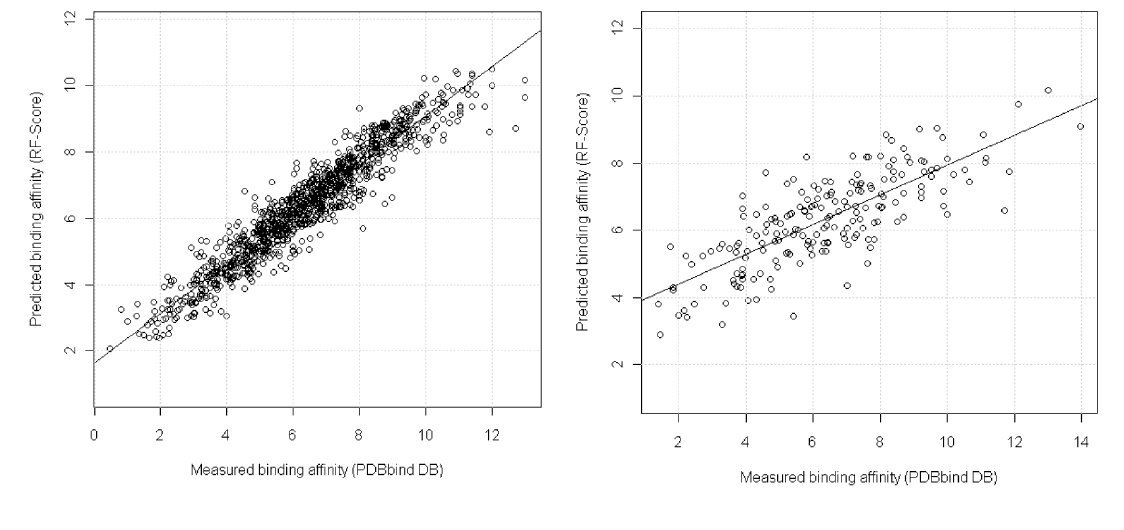
\includegraphics[width=17cm]{imagens/treino_teste_ballester.png}
	\caption{Treino E Teste com Random Forests}
	\end{figure}
\newline
Treinamento utilizando 1105 amostras obteve um RMSE=0.74.
\newline
Teste utilizando 195 amostras obteve um RMSE=1.58.

\section{Resultados do SVM}

Ao utilizar svm como alternativa neste trabalho foi possível obter tais resultados:
    \begin{figure}[h]
	\centering
	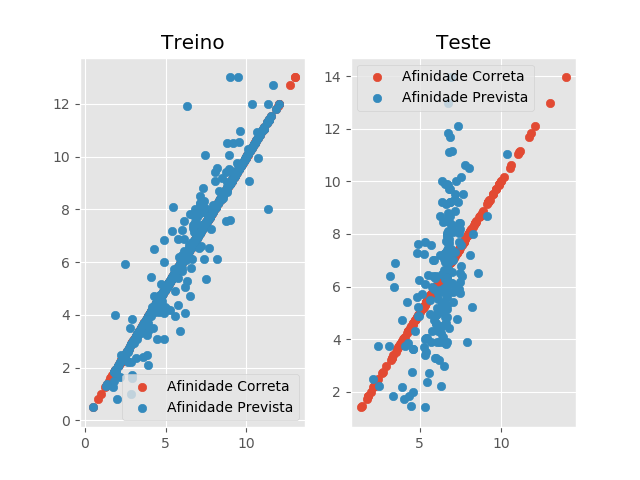
\includegraphics[width=17cm]{imagens/teste_treino_meu.png}
	\caption{Treino E Teste com SVM}
	\end{figure}
\newline
Treino com 1105 amostras refinidas obteve um RMSE de 0.45.
\newline
Teste com 195 amostras brutas obteve um RMSE de 1.97.

\section{SVM X Random Forest}
Ao utilizar a técnica de Random Forest nota-se que o RMSE é menor no teste, isso caracteriza menor índice de erros e consequentemente melhores resultados preditos.

Diferentemente no SVM, percebe-se que a previsão para de treinamento foi superior,rmse=0.45 (SVM) contra 0.74(florestas aleatórias) embora isso não seja tão relevante.
Já que no teste ouve uma maior falha ao prever resultados, com 1.97 do svm contra 1.58 das florestas aleatórias.

Em resumo, o trabalho proposto por \citeauthor{ballester2010machine} é melhor para predição de valores de afinidade dos complexos do tipo proteína-ligante, e consequentemente, é melhor para poder aplicar uma função de pontuação em algum software futuro.

\chapter{Conclusões}

Colocar toda análise de cada capítulo aqui desde a introdução,fundamentação teórica,metodologia e resultados.

Conforme foi visto ao longo deste trabalho, sempre irão existir avanços que possibilitem o uso de novas tecnologias, neste trabalho em especial, no docking molecular.
Neste trabalho foi feito um estudo de diversas áreas; biomedicina, inteligência artificial, programação e estatística. Todas com a finalidade de otimizar a predição de afinidade dos complexos do tipo ligante-proteína.
Não foi possível superar o algoritmo de florestas aleatórias de \citeauthor{ballester2010machine}, que possui um RMSE=1.58, com o algoritmo de SVM realizado neste trabalho que obteve RMSE=1.97.
Em contra-ponto, foi explorado e testado diversos kernels e parâmetros do SVM, do qual serviu para aumentar o nível de conhecimento elucidado para elaboração de futuros estudos. 


\section{Trabalhos Futuros}

Apesar de ter todo esforço e evolução da área de inteligência artificial, muito falta para ser alcançado, a extração de informações ainda é pequena e bastante heterogênea para um processamento avançado, o que traz por consequência uma falha muito grande em prever resultados reais para aplicações da biomedicina no dia-a-dia.
Para um novo trabalho, deverá ser explorado outra técnica de aprendizado de máquina que apresente melhores resultados, como o uso de Redes Neurais profundas, contando com mais informações presentes em bases de dados mais recentes, para que dessa forma ocorra uma melhora significativa no treinamento e teste, prevendo melhores resultados.

\bibliography{relatorio}
\bibliographystyle{abnt}

%\appendix

\end{document}

